%%%%%%%%%%%%%%%%%%%%%%%%%%%%%%%%%%%%%%%%%%%%%%%%%%%%%%%%%%%%%%%%%%%%%%%%%%%%%%%%%%%%%%%%%%%%%%%%%%%%%
% Plantilla básica de Latex en Español.
%
% Autor: Andrés Herrera Poyatos (https://github.com/andreshp)
%
% Es una plantilla básica para redactar documentos. Utiliza el paquete fancyhdr para darle un
% estilo moderno pero serio.
%
% La plantilla se encuentra adaptada al español.
%
%%%%%%%%%%%%%%%%%%%%%%%%%%%%%%%%%%%%%%%%%%%%%%%%%%%%%%%%%%%%%%%%%%%%%%%%%%%%%%%%%%%%%%%%%%%%%%%%%%%%%%

%-----------------------------------------------------------------------------------------------------
%	INCLUSIÓN DE PAQUETES BÁSICOS
%-----------------------------------------------------------------------------------------------------

\documentclass{article}

\usepackage{lipsum}                     % Texto dummy. Quitar en el documento final.

%-----------------------------------------------------------------------------------------------------
%	SELECCIÓN DEL LENGUAJE
%-----------------------------------------------------------------------------------------------------

% Paquetes para adaptar Látex al Español:
\usepackage[spanish,es-noquoting, es-tabla, es-lcroman]{babel} % Cambia
\usepackage[utf8]{inputenc}                                    % Permite los acentos.
\selectlanguage{spanish}                                       % Selecciono como lenguaje el Español.

%-----------------------------------------------------------------------------------------------------
%	SELECCIÓN DE LA FUENTE
%-----------------------------------------------------------------------------------------------------

% Fuente utilizada.
\usepackage{courier}                    % Fuente Courier.
\usepackage{microtype}                  % Mejora la letra final de cara al lector.

%-----------------------------------------------------------------------------------------------------
%	ESTILO DE PÁGINA
%-----------------------------------------------------------------------------------------------------

% Paquetes para el diseño de página:
\usepackage{fancyhdr}               % Utilizado para hacer títulos propios.
\usepackage{lastpage}               % Referencia a la última página. Utilizado para el pie de página.
\usepackage{extramarks}             % Marcas extras. Utilizado en pie de página y cabecera.
\usepackage[parfill]{parskip}       % Crea una nueva línea entre párrafos.
\usepackage{geometry}               % Asigna la "geometría" de las páginas.

% Se elige el estilo fancy y márgenes de 3 centímetros.
\pagestyle{fancy}
\geometry{left=3cm,right=3cm,top=3cm,bottom=3cm,headheight=1cm,headsep=0.5cm} % Márgenes y cabecera.
% Se limpia la cabecera y el pie de página para poder rehacerlos luego.
\fancyhf{}

% Espacios en el documento:
\linespread{1.1}                        % Espacio entre líneas.
\setlength\parindent{0pt}               % Selecciona la indentación para cada inicio de párrafo.

% Cabecera del documento. Se ajusta la línea de la cabecera.
\renewcommand\headrule{
	\begin{minipage}{1\textwidth}
	    \hrule width \hsize
	\end{minipage}
}

% Texto de la cabecera:
\lhead{\docauthor}                          % Parte izquierda.
\chead{}                                    % Centro.
\rhead{\subject \ - \doctitle}              % Parte derecha.

% Pie de página del documento. Se ajusta la línea del pie de página.
\renewcommand\footrule{
\begin{minipage}{1\textwidth}
    \hrule width \hsize
\end{minipage}\par
}

\lfoot{}                                                 % Parte izquierda.
\cfoot{}                                                 % Centro.
\rfoot{Página\ \thepage\ de\ \protect\pageref{LastPage}} % Parte derecha.


%-----------------------------------------------------------------------------------------------------
%	PORTADA
%-----------------------------------------------------------------------------------------------------

% Elija uno de los siguientes formatos.
% No olvide incluir los archivos .sty asociados en el directorio del documento.
\usepackage{title1}
%\usepackage{title2}

%-----------------------------------------------------------------------------------------------------
%	TÍTULO, AUTOR Y OTROS DATOS DEL DOCUMENTO
%-----------------------------------------------------------------------------------------------------

% Título del documento.
\newcommand{\doctitle}{Práctica 3}
% Subtítulo.
\newcommand{\docsubtitle}{Modelos jerárquicos}
% Fecha.
\newcommand{\docdate}{3 \ de \ Diciembre \ de \ 2016}
% Asignatura.
\newcommand{\subject}{Informática Gráfica}
% Autor.
\newcommand{\docauthor}{Nuria Rodríguez Barroso}
\newcommand{\docaddress}{Universidad de Granada}
\newcommand{\docemail}{rbnuria6@gmail.com}

%-----------------------------------------------------------------------------------------------------
%	RESUMEN
%-----------------------------------------------------------------------------------------------------

% Resumen del documento. Va en la portada.
% Puedes también dejarlo vacío, en cuyo caso no aparece en la portada.
%\newcommand{\docabstract}{}
%\newcommand{\docabstract}{En este texto puedes incluir un resumen del documento. Este informa al lector sobre el contenido del texto, indicando el objetivo del mismo y qué se puede aprender de él.}

\begin{document}

%\maketitle

%-----------------------------------------------------------------------------------------------------
%	ÍNDICE
%-----------------------------------------------------------------------------------------------------

% Profundidad del Índice:
%\setcounter{tocdepth}{1}

%\newpage
%\tableofcontents
%\newpage

%-----------------------------------------------------------------------------------------------------
%	SECCIÓN 1
%-----------------------------------------------------------------------------------------------------

\section{Grafo de escena}

Para facilitar la representación del esquema, cuando introduzcamos en una casilla el nombre de otra clase del esquema en cursiva será equivalente a una flecha de dicha otra clase a la casilla en cuestión.

\begin{table}[h]
	\centering
	\label{1}
	\begin{tabular}{|c|}
		\hline
		\textbf{Bender}\\ \hline
		Tras(dist\_lateral, 0, dist\_lineal)\\ \hline
		Esc(0.1, 0.1, 0.1)\\ \hline
		\textit{Cuerpo}\\ \hline
		\textit{Cabeza}\\ \hline
		Tras(0.6, 5.5, 0)\\ \hline
		\textit{Pierna}\\ \hline
		Tras(-1.2, 0, 0)\\ \hline
		\textit{Pierna}\\ \hline
		Tras(0.6, 0, 0)\\ \hline
		\textit{Brazo\_Derecho}\\ \hline
		\textit{Brazo\_Izquierdo}\\ \hline

	\end{tabular}
\end{table}

\begin{table}[h]
	\centering
	\label{2}
	\begin{tabular}{|c|}
		\hline
		\textbf{Cuerpo}\\ \hline
		Esc(2,2,2)\\ \hline
		Tras(0, 3.7, 0)\\ \hline
		\textit{Cilindro\_deforme}\\ \hline

	\end{tabular}
\end{table}



\begin{table}[h!]
	\centering
	\label{4}
	\begin{tabular}{|c|}
		\hline
		\textbf{Cabeza}\\ \hline
		Tras(0, 9.4, 0)\\ \hline
		Esc(2, 2, 2)\\ \hline
		\textit{Cuello}\\ \hline
		Esc( 0.5, 0.5, 0.5)\\ \hline
		Tras(0, 1.5, 0)\\ \hline
		Rot(15*angulo,0,1,0)\\ \hline
		\textit{Cilindro}\\ \hline
		Tras(0,1,0)\\ \hline
		\textit{Ojo}\\ \hline
		Tras(-1, 0, 0)\\ \hline
		\textit{Ojo}\\ \hline
		Tras(0.5, 0, -1)\\ \hline
		Tras(0, 1, 0)\\ \hline
		Esc(0.05, 0.1, 0.1)\\ \hline
		Rot(180,1,0,0)\\ \hline
		\textit{Cono}\\ \hline
		Esc(20,10,10)\\ \hline
		Tras(0, -1.2, 0)\\ \hline
		Esc(0.15, 0.15, 0.15)\\ \hline
		\textit{Esfera}\\ \hline
	\end{tabular}
\end{table}

\begin{table}[h!]
	\centering
	\label{3}
	\begin{tabular}{|c|}
		\hline
		\textbf{Ojo}\\ \hline
		Rot(90, 1, 0, 0)\\ \hline
		Esc(0.25, 0.25, 0.25)\\ \hline
		\textit{Semiesfera}\\ \hline
	\end{tabular}
\end{table}



\begin{table}[h!]
	\centering
	\label{5}
	\begin{tabular}{|c|}
		\hline
		\textbf{Pierna}\\ \hline
		Esc(0.5, 0.5, 0.5)\\ \hline
		Tras(0, -1, 0)\\ \hline
		\textit{Cilindro\_deforme}\\ \hline
		Tras(0,-2,0)\\ \hline
		\textit{Cilindro\_deforme}\\ \hline
		Tras(0,-2,0)\\ \hline
		\textit{Cilindro\_deforme}\\ \hline
		Tras(0,-2,0)\\ \hline
		\textit{Cilindro\_deforme}\\ \hline
		Tras(0,-2,0)\\ \hline
		Esc(2, 2, 2)\\ \hline
		\textit{Semiesfera}\\ \hline
	\end{tabular}
\end{table}

\begin{table}[h!]
	\centering
	\label{6}
	\begin{tabular}{|c|}
		\hline
		\textbf{Brazo\_Derecho}\\ \hline
		Esc(0.4, 0.4, 0.4)\\ \hline
		Tras(5.2, 8, 0)\\ \hline
		Rot(-10*angulo,0,1,0)\\ \hline
		Esc(1, proporción, 1)\\ \hline
		\textit{Cilindro}\\ \hline
		Tras(0, 2*(proporción), 0)\\ \hline
		\textit{Cilindro}\\ \hline
		Tras(0, 2*(proporción), 0)\\ \hline
		\textit{Cilindro}\\ \hline
		Tras(0, 2*(proporción), 0)\\ \hline
		Tras(0, 0.5, 0)\\ \hline
		Rot(180, 1, 0, 0)\\ \hline
		Esc(1, 2, 2)\\ \hline
		\textit{Semiesfera}\\ \hline
	\end{tabular}
\end{table}


\begin{table}[h!]
	\centering
	\label{7}
	\begin{tabular}{|c|}
		\hline
		\textbf{Brazo\_Izquierdo}\\ \hline
		Esc(0.4, 0.4, 0.4)\\ \hline
		Tras(-5.2, 8, 0)\\ \hline
		Rot(10*angulo,0,1,0)\\ \hline
		Esc(1, proporción, 1)\\ \hline
		\textit{Cilindro}\\ \hline
		Tras(0, 2*(proporción), 0)\\ \hline
		\textit{Cilindro}\\ \hline
		Tras(0, 2*(proporción), 0)\\ \hline
		\textit{Cilindro}\\ \hline
		Tras(0, 2*(proporción), 0)\\ \hline
		Tras(0, 0.5, 0)\\ \hline
		Rot(180, 1, 0, 0)\\ \hline
		Esc(1, 2, 2)\\ \hline
		\textit{Semiesfera}\\ \hline
	\end{tabular}
\end{table}

\begin{table}[h!]
	\centering
	\label{8}
	\begin{tabular}{|c|}
		\hline
		\textbf{Semiesfera}\\ \hline
		Clase derivada de MallaInd\\ \hline
	\end{tabular}
\end{table}

\begin{table}[h!]
	\centering
	\label{9}
	\begin{tabular}{|c|}
		\hline
		\textbf{Esfera}\\ \hline
		Clase derivada de MallaInd\\ \hline
	\end{tabular}
\end{table}

\begin{table}[h!]
	\centering
	\label{10}
	\begin{tabular}{|c|}
		\hline
		\textbf{Cuello}\\ \hline
		Clase derivada de MallaInd\\ \hline
	\end{tabular}
\end{table}

\begin{table}[h!]
	\centering
	\label{11}
	\begin{tabular}{|c|}
		\hline
		\textbf{Cilindro}\\ \hline
		cilindro.ply\\ \hline
	\end{tabular}
\end{table}


\begin{table}[h!]
	\centering
	\label{12}
	\begin{tabular}{|c|}
		\hline
		\textbf{Cilindro\_deforme}\\ \hline
		cilindro\_deforme.ply\\ \hline
	\end{tabular}
\end{table}



\cleardoublepage
\section{Lista de grados de libertad}
	En total contaremos con cinco grados de libertad (aunque dos son muy parecidos, por lo que en realidad serían cuatro tipos de movimientos) que detallaremos a continuación. Para cambiar de un grado de libertad a otro utilizaremos la tecla 'G', la cual variará la variable $p3\_grado\_libertad\_activo$. Dependiendo del valor de esta variable podemos encontrar:
	 
	 
	 
	\subsection{Grado de libertad 0: Girar la cabeza}
	
	\begin{figure*}[h]
		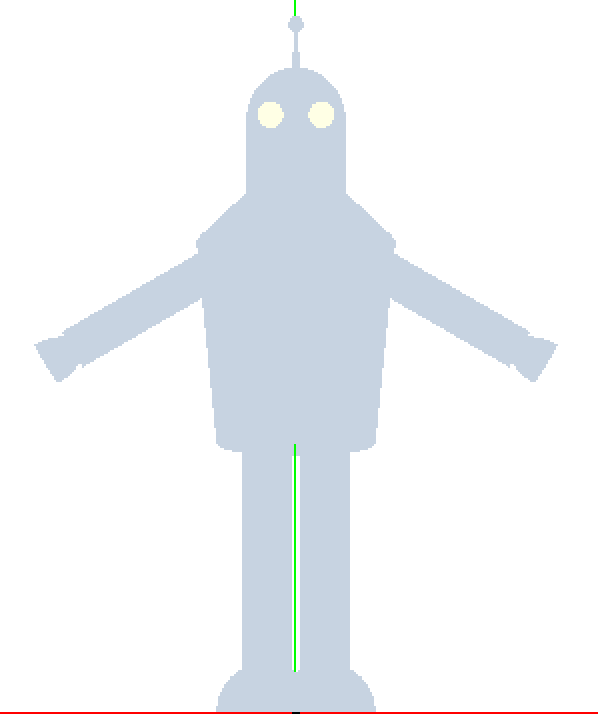
\includegraphics[width=0.4\linewidth]{cabeza1}
		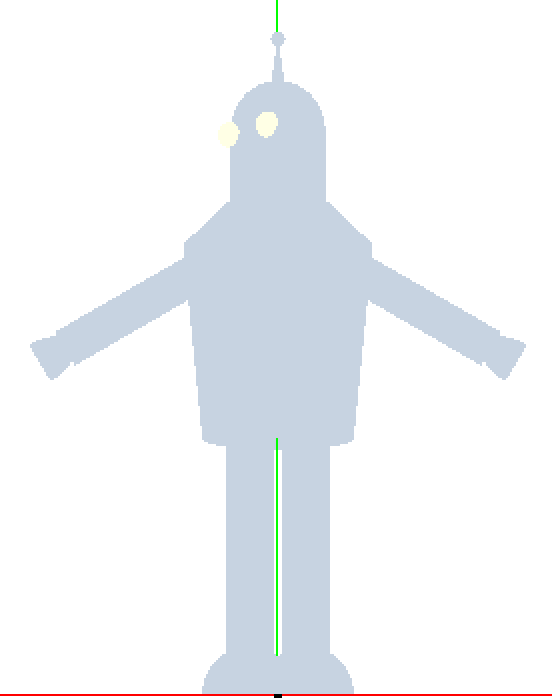
\includegraphics[width=0.38\linewidth]{cabeza2}
		\caption{Sin aplicar movimiento.}
		\caption{Con una rotación de cabeza.}
		\label{fig:cabeza}
	\end{figure*}
	
	
	En este grado de libertad, $Bender$ girará la cabeza de derecha a izquierda llegando a mover 90º desde la posición inicial (mirando al frente) a cada uno de los lados.
	
	\begin{itemize}
		\item \textbf{Tipo de nodo: } Cabeza. 
		\item \textbf{Método que lo modifica: } Lo modifica el método \textit{void girar\_cabeza(float angulo)} de la clase \textit{Bender}, que a su vez llama al método \textit{void girar(float angulo)} de la clase \textit{Cabeza}.
		\item \textbf{Nodo del grafo al que afecta: } Afecta al nodo 5 del grafo, que se corresponde con una matriz de rotación. 
		\item \textbf{Transformación asociada: } Una rotación de ángulo dado.
		\item \textbf{Atributos del parámetro: }
		\begin{enumerate} 
			\item \textit{descripción: } `'Girar cabeza''
			\item  \textit{valor\_inicial:} 0
			\item \textit{incremento: } 0.1
			\item \textit{valor\_mínimo: } -5
			\item \textit{valor\_máximo: } 5
			\item \textit{velocidad\_inicial: } 1
			\item \textit{aceleración: } 2
			\item \textit{magnitud\_máxima\_aceleración: }  8
		\end{enumerate}
	\end{itemize}


	\subsection{Grado de libertad 1: Desplazamiento lateral}
	
	\begin{figure*}[h]
		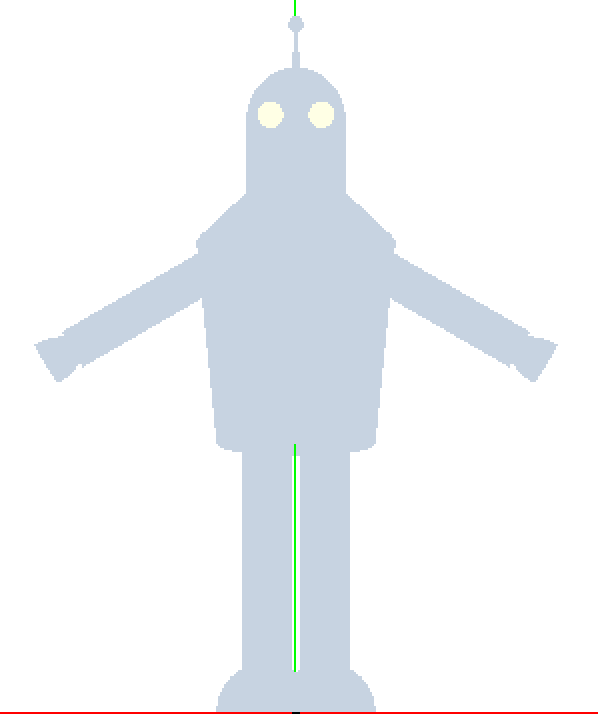
\includegraphics[width=0.4\linewidth]{cabeza1}
		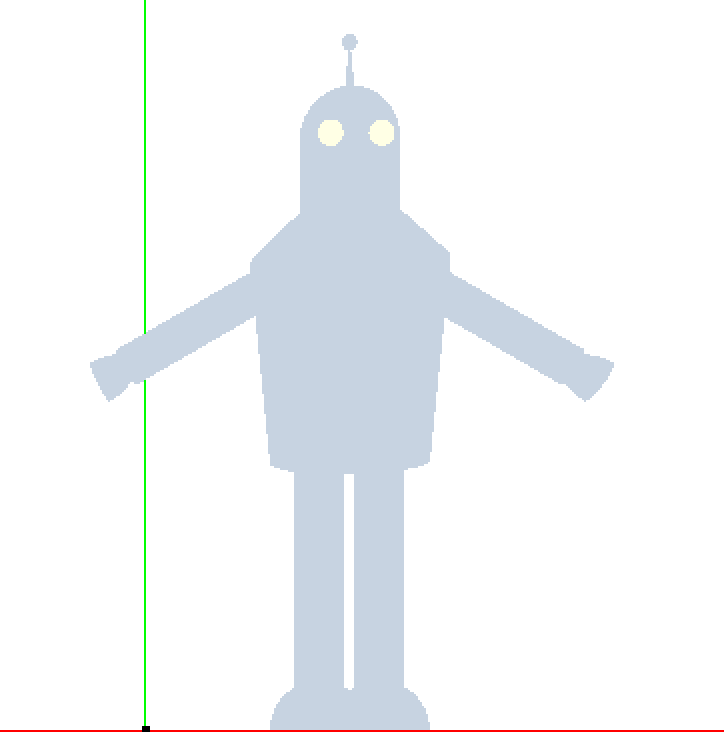
\includegraphics[width=0.47\linewidth]{desplazamientolateral}
		\caption{Sin aplicar movimiento.}
		\caption{Aplicado desplazamiento lateral.}
		\label{fig:desplazamientolateral}
	\end{figure*}

	En este grado de libertad, \textit{Bender} se desplaza lateralmente (sobre el eje x) de izquierda a derecha con unos máximos (que detallaremos a continuación).
	
	\begin{itemize}
		\item \textbf{Tipo de nodo: } Bender 
		\item \textbf{Método que lo modifica: } Lo modifica el método \textit{void desplazarse\_lateralmente(float distancia)} de la clase \textit{Bender}.
		\item \textbf{Nodo del grafo al que afecta: } Afecta al nodo 0 del grafo (primer nodo), siendo este una matriz de traslación que afecta a todo el dibujo de \textit{Bender} que le sigue.
		\item \textbf{Transformación asociada: } Traslación.
		\item \textbf{Atributos del parámetro: }
		\begin{enumerate}
			\item \textit{descripción: } `'Desplazamiento lateral''
			\item  \textit{valor\_inicial:} 0
			\item \textit{incremento: } 0.01
			\item \textit{valor\_mínimo: } -1
			\item \textit{valor\_máximo: } 1
			\item \textit{velocidad\_inicial: } 1
			\item \textit{aceleración: } 2
			\item \textit{magnitud\_máxima\_aceleración: }  8
		\end{enumerate}
	\end{itemize}


	\subsection{Grado de libertad 2: Desplazamiento lineal hacia delante.}
	
	\begin{figure*}[h]
		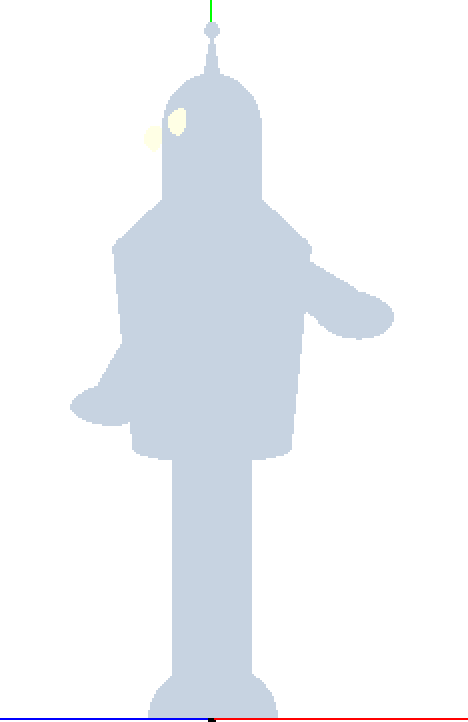
\includegraphics[width=0.34\linewidth]{haciadelante1}
		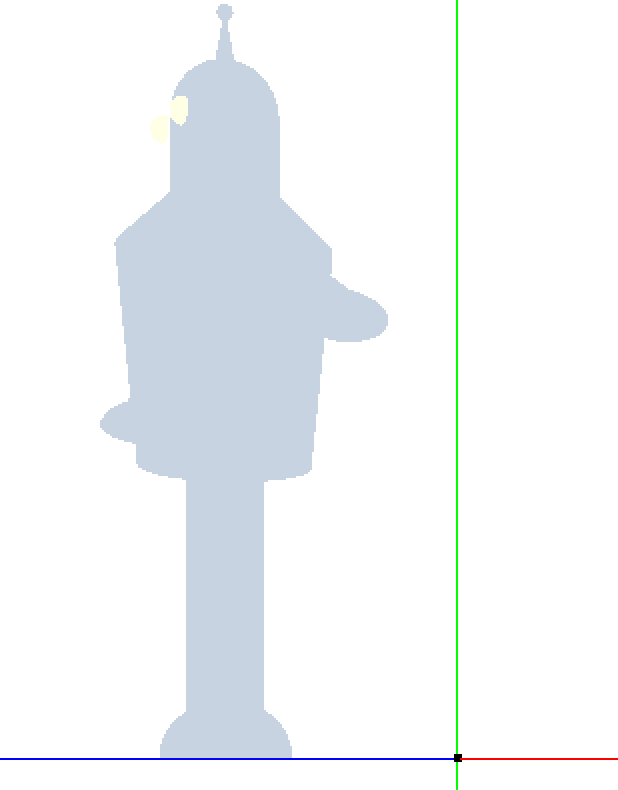
\includegraphics[width=0.42\linewidth]{haciadelante2}
		\caption{Sin aplicar movimiento.}
		\caption{Con un desplazamiento hacia delante.}
		\label{fig:haciadelante}
	\end{figure*}
	
	Similar al grado de libertad 2, con este movimiento \textit{Bender} se desplaza por el eje z dando la sensación de que se desplaza hacia delante y hacia detrás.
	
	\begin{itemize}
		\item \textbf{Tipo de nodo: } Bender.
		\item \textbf{Método que lo modifica: } Lo modifica el método \textit{void desplazamiento\_lineal(float distancia)} de la clase \textbf{Bender}.
		\item \textbf{Nodo del grafo al que afecta: } Afecta al nodo 0, que es una matriz de traslación que afecta a todo el dibujo del mismo. 
		\item \textbf{Transformación asociada: } Traslación.
		\item \textbf{Atributos del parámetro: }
		\begin{enumerate}
			\item \textit{descripción: } `'Desplazamiento lineal ''
			\item  \textit{valor\_inicial:} 0
			\item \textit{incremento: } 0.01
			\item \textit{valor\_mínimo: } -1
			\item \textit{valor\_máximo: } 1
			\item \textit{velocidad\_inicial: } 1
			\item \textit{aceleración: } 2
			\item \textit{magnitud\_máxima\_aceleración: }  8
		\end{enumerate}
	\end{itemize}


	\subsection{Grado de libertad 3: Saludo.}
	
		\begin{figure*}[h]
			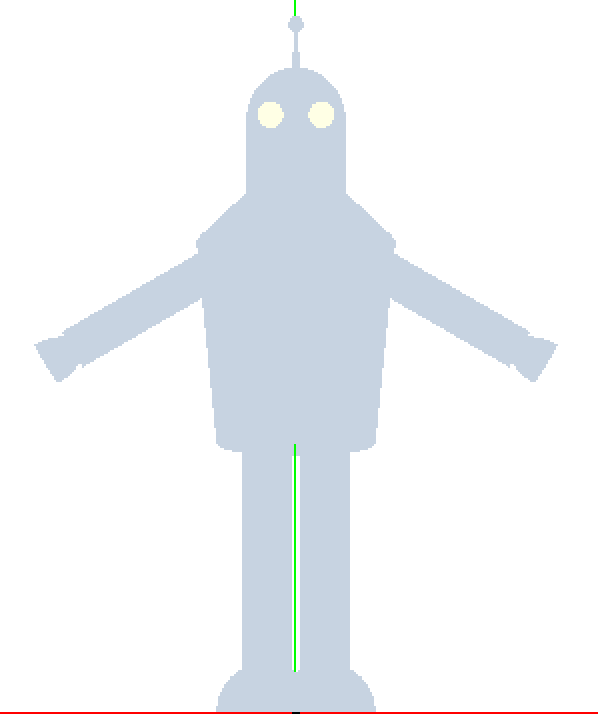
\includegraphics[width=0.4\linewidth]{cabeza1}
			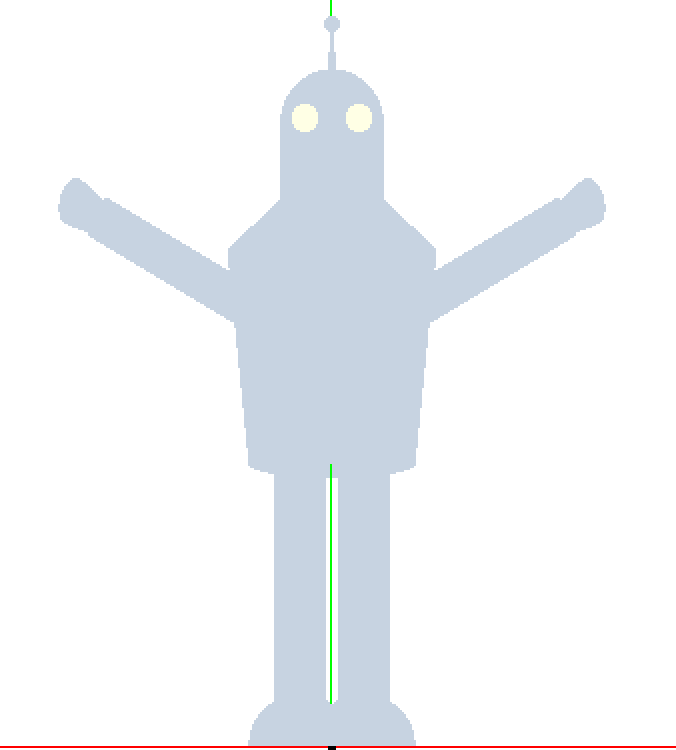
\includegraphics[width=0.42\linewidth]{saludo}
			\caption{Sin aplicar movimiento.}
			\caption{Con saludo aplicado.}
			\label{fig:saludo}
		\end{figure*}

	Este grado de libertad llamado '`Saludo'', consiste en el movimiento de los brazos de forma que parezca que \textit{Bender} está saludando.
	
	\begin{itemize}
		\item \textbf{Tipo de nodo: } Brazo\_izquierdo y Brazo\_derecho.
		\item \textbf{Método que lo modifica: } Lo modifica el método \textit{void saludar(float angulo)} de la clase \textit{Bender}, que a su vez llama al método \textit{void mover(float angulo)} de cada una de las subclases Brazo\_derecho y Brazo\_izquierdo.
		\item \textbf{Nodo del grafo al que afecta: } Afecta al nodo 2, que es una matriz de rotación que añadirá una rotación en función de un ángulo pasado como argumento.
		\item \textbf{Transformación asociada: } Rotación.
		\item \textbf{Atributos del parámetro: }
		\begin{enumerate}
			\item \textit{descripción: } `'Saludo''
			\item  \textit{valor\_inicial:} 12
			\item \textit{incremento: } 0.1
			\item \textit{valor\_mínimo: } 6
			\item \textit{valor\_máximo: } 12
			\item \textit{velocidad\_inicial: } 1
			\item \textit{aceleración: } 2
			\item \textit{magnitud\_máxima\_aceleración: }  8
		\end{enumerate}
	\end{itemize}

	\subsection{Grado de libertad 3: Estirar los brazos.}
	
		\begin{figure*}[h]
		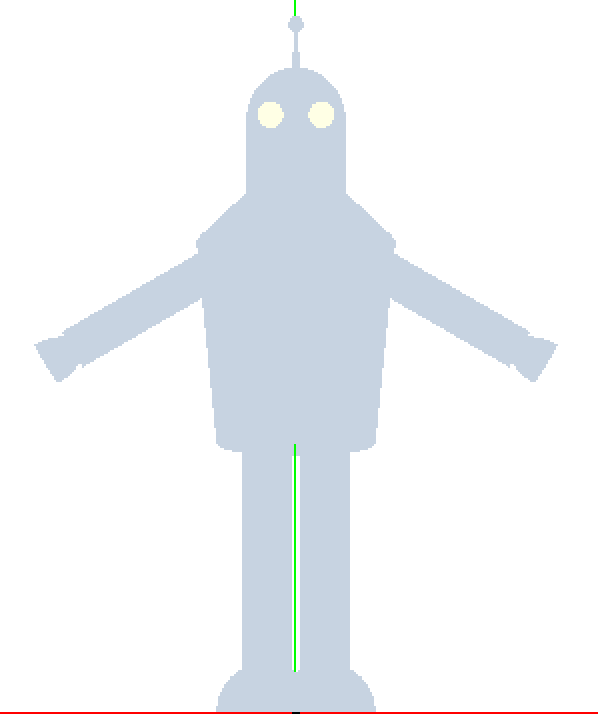
\includegraphics[width=0.4\linewidth]{cabeza1}
		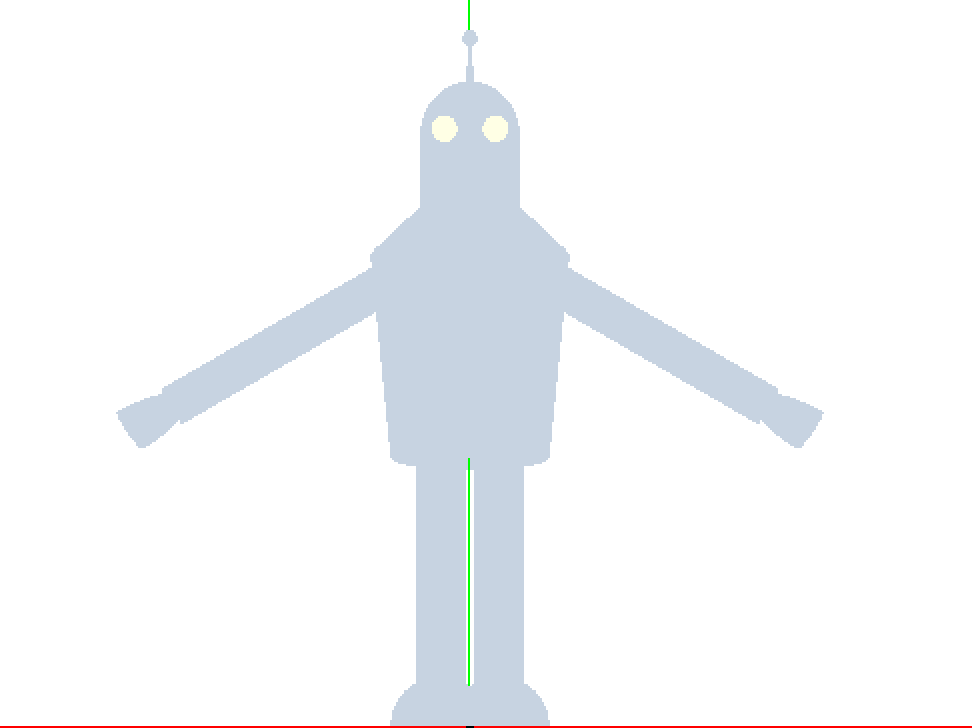
\includegraphics[width=0.65\linewidth]{estirarbrazos}
		\caption{Sin aplicar movimiento.}
		\caption{Con brazos estirados.}
		\label{fig:estirarbrazos}
	\end{figure*}

	Este grado de libertad llamado '`estirar brazos'', consiste en la expansión de los brazos de forma que aumenten su tamaño (se estiren).
	
	\begin{itemize}
		\item \textbf{Tipo de nodo: } Brazo\_izquierdo y Brazo\_derecho.
		\item \textbf{Método que lo modifica: } Lo modifica el método \textit{void estirar\_brazos(float proporcion)} de la clase \textit{Bender}, que a su vez llama al método \textit{void estirar(float proporcion)} de cada una de las subclases Brazo\_derecho y Brazo\_izquierdo.
		\item \textbf{Nodo del grafo al que afecta: } Afecta al nodo 3, que es una matriz de escalado, que añadirá un escalado en la coordenada de la y (solo alargará), cada uno de los cilindros que componen los brazos de \textit{Bender}.
		\item \textbf{Transformación asociada: } Escalado.
		\item \textbf{Atributos del parámetro: }
		\begin{enumerate}
			\item \textit{descripción: } `'Estirar brazos''
			\item  \textit{valor\_inicial:} 1
			\item \textit{incremento: } 0.01
			\item \textit{valor\_mínimo: } 1
			\item \textit{valor\_máximo: } 2
			\item \textit{velocidad\_inicial: } 2
			\item \textit{aceleración: } 2
			\item \textit{magnitud\_máxima\_aceleración: }  4
		\end{enumerate}
	\end{itemize}






\end{document}